\chapter{The Stern-Gerlach Experiment}

\section{Spin Angular Momentum}

Let's start with a system that is pretty much as far away from the quantum world as possible -- the Earth and Sun.  With its total motion, the Earth has two kinds of angular momentum:  \emph{orbital} angular momentum $\vec{L}$ from its orbit around the sun, and \emph{spin} angular momentum $\vec{S}$, resulting from its 24 hour rotation.  Of course, the spin angular momentum in this case is due to adding up the orbital angular momentum $\vec{L}_i = \vec{r}_i \times \vec{p}_i$ of each of the tiny pieces of the Earth, but we'll keep the distinction because this is definitively not the case in quantum systems as we'll see.  Note that the two kinds of angular momentum for the Earth point in different directions since the rotation axis of the Earth is tilted 23$^\circ$ from the orbital plane.

As a simple quantum system, consider an electron in orbit around a proton -- a hydrogen atom.  The electron has orbital angular momentum just like the Earth (depending on what state it's in), and it also has spin angular momentum.  Careful, though, as the electron doesn't rotate like the Earth -- how can it when it has essentially no size or diameter to spin?  Despite this, it has measurable intrinsic angular momentum, which we'll call \emph{spin} $\vec{S}$.  Since spin is a vector, it has components $(S_x, S_y, S_z)$, and thus to specify the spin of the electron we need to use three different numbers; keep this in mind for later.

Suppose we put a stationary electron in a magnetic field $\vec{B}$.  Since the electron is stationary, the Lorentz force
\[
\vec{F} = q\vec{v} \times \vec{B}
\]
is zero.  But the electron's spin angular momentum gives it a magnetic dipole moment $\vec{\mu}$, and it's then possible for an \emph{inhomogeneous} magnetic field to exert a force (see Griffiths \emph{Introduction to Electrodynamics}, fourth edition, section 6.2)
\begin{equation}
\vec{F} = \grad (\vec{\mu} \cdot \vec{B}).
\label{eq_force_inhomo}
\end{equation}

\begin{figure}
\centering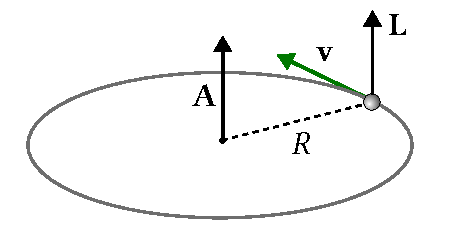
\includegraphics[width=0.5\linewidth]{Figures/Chapter 1/fig_circular_orbit.pdf}
\caption{A charged particle in a circular orbit has a magnetic dipole moment.}
\label{fig_circular_orbit}
\end{figure}

We can calculate the magnetic dipole moment due to orbital angular momentum easily enough; Figure \ref{fig_circular_orbit} shows a particle in a circular orbit of radius $R$ and circular velocity $\vec{v}$.  If we think of this as a current loop, the dipole moment is just the current $I$ times the area $\vec{A}$,
\[
\vec{\mu} = I\vec{A}.
\]
The magnitude of the area vector is just $A = \pi R^2$m and the direction is perpendicular to the orbit, while the current will be the charge divided by the time it takes for the charge to make the orbit:
\[
I = \frac{q}{T} = \frac{q}{2\pi R / v}.
\]
The dipole moment is then
\[
\vec{\mu} = \left( \frac{1}{2} qvR, \text{ perpendicular to the orbit} \right).
\]
It's more useful, though, to put this in terms of the angular momentum $\vec{L} = \vec{r} \times \vec{p}$, which for a circular orbit is
\[
\vec{L} = \left( rmv, \text{ perpendicular to the orbit} \right).
\]
Finally, then, the magnetic dipole moment arising from orbital angular momentum is 
\begin{equation}
\vec{\mu} = \frac{q}{2m} \vec{L}.
\end{equation}

Things are slightly different for the spin angular momentum of a charged particle.  We can still think of the magnetic dipole moment as coming from a current loop, but we have to write 
\begin{equation}
\vec{\mu} = \frac{gq}{2m} \vec{S},
\end{equation}
where $g$ is called the gyroscopic ratio or often just ``$g$-factor'' and, for an electron, is \emph{almost} $g = 2$.\footnote{We don't need to worry about this here, but each charged particle with spin has its own $g$-factor -- the proton has $g = 5.58$, for example.  These can be measuring and in some cases calculated theoretically, but it requires quantum field theory to do it properly.}

Let's go back to the idea of putting an electron in an inhomogeneous field, and we'll suppose that the field is constant in the $x$ and $y$ directions but changes along the $z$ direction.  Then, with no orbital motion,
\[
\vec{\mu} \cdot \vec{B} = \mu_x B_x + \mu_y B_y + \mu_z B_z,
\]  
and since the first two terms are constant, equation (\ref{eq_force_inhomo}) gives
\begin{equation}
\vec{F} = \grad ( \mu_z B_z ) = \mu_z \dfdx{B_z}{z} \, \hat{z} = \frac{gq}{2m} \dfdx{B_z}{z} S_z \, \hat{z}.
\label{eq_force_spin}
\end{equation}
The force on the electron in this case is directed along the $z$ direction and proportional to the component of spin angular momentum along that direction -- the more the spin aligns with the $z$ axis, the greater the force.
%
%
%

\section{The Stern-Gerlach Experiment}

In 1922 Otto Stern and Walther Gerlach used these ideas to measure the spin angular momentum of electrons.  Their experiment is shown in Figure \ref{fig_stern_gerlach_exp}, and they actually used silver atoms rather than electrons.  Why silver?  The atoms are electrically neutral, so there won't be any direct magnetic force on the atoms from the magnetic field, and the electronic configuration of silver is $1s^22s^22p^63s^23p^64s^23d^{10}4p^64d^{10}5s^1$.  Except for the outermost electron, all others are in closed shells, meaning we can ignore their contribution to the angular momentum of the silver atom.  The outermost electron is in an $s$-orbit, which has no orbital angular momentum -- so the only angular momentum of the entire silver atom is due to the spin of that one outer electron.

\begin{figure}
\centering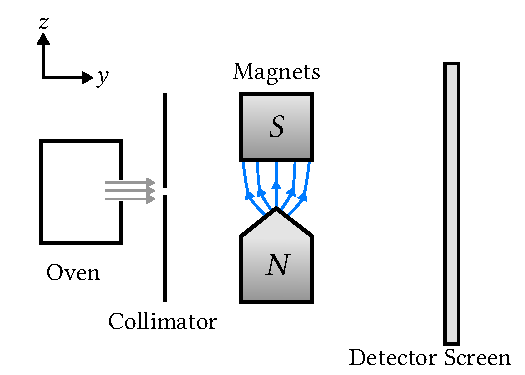
\includegraphics[width=0.6\linewidth]{Figures/Chapter 1/fig_stern_gerlach_exp.pdf}
\caption{The Stern-Gerlach experiments, in which silver atoms are deflected by an inhomogeneous magnetic field.}
\label{fig_stern_gerlach_exp}
\end{figure}

The Stern-Gerlach experiment proceeds as follows.  First, the oven boils silver atoms off of a solid piece of silver; the atoms are ``thermalized,'' meaning they come out in all directions and with random spin orientations.  A collimating slit produces a narrow beam of these atoms which pass between the magnets.  The magnets are constructed to create an inhomogeneous magnetic field, with the inhomogeneity in the $z$ direction; note that as shown the magnetic field gets stronger in the negative $z$ direction, so $\partial B_z / \partial z$ is negative in equation (\ref{eq_force_spin}).  Because the charge on the electron is negative as well, the force on a silver atom passing through the field will be up along $z$ if the spin has a positive $z$ component, and down along $-z$ if the spin has a negative $z$ component.  Finally, the deflection of each atom is measured when they hit the detecting screen.

What do we expect?  Well, as mentioned above, the oven thermalizes the atoms so the spin of the outer electron is in random directions.  That means the force on each atom will be random as well -- some atoms will get pushed up, some will get pushed down, and each with varying strength (up to some maximum for those spins that are entirely along $z$ or $-z$).  This expected result is shown in Figure \ref{fig_stern_gerlach_result_expected} (a).

\begin{figure}
\centering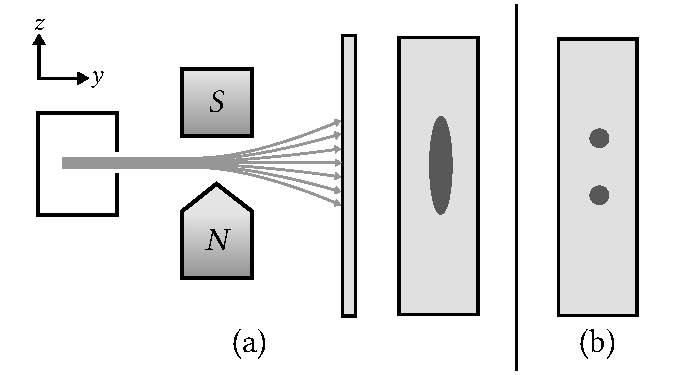
\includegraphics[width=0.8\linewidth]{Figures/Chapter 1/fig_stern_gerlach_result_expected.pdf}
\caption{(a) Classically expected result.  (b) Actual result showing quantization of spin angular momentum.}
\label{fig_stern_gerlach_result_expected}
\end{figure}

But that's not at all what Stern and Gerlach saw; instead, as Figure \ref{fig_stern_gerlach_result_expected} (b) shows, they detected only two locations where silver atoms hit the screen, corresponding to spin angular momentum values of either 
\[
S_z = +\frac{\hbar}{2} \quad \text{or} \quad S_z = -\frac{\hbar}{2}.
\]
This is clear evidence of the \emph{quantization} of angular momentum, something Niels Bohr suggested in 1913 when developing his model of the atom.

%
%
%

\section{Extending the Experiments}

Before we discuss this further, I want to introduce some notation:
\begin{equation}
\label{eq_ket_definition}
\boxed{
\ket{\psi} \rightarrow \text{ Represents the state of a quantum mechanical system.}
}
\end{equation}
This notation is often called a ``ket,'' for reasons we'll see later, and it includes all possible information you could know about a particular quantum system.  Consider, for example, a silver atom that has been measured to have $S_z = +\hbar/2$.  We could represent the state of the atom by 
\[
\ket{+} \rightarrow \text{ State for which $S_z = +\hbar/2$ has been measured},
\]
although it's also common to use $\ket{\uparrow}$ or $\ket{+z}$.  This state is usually called ``spin up.''  Similarly, the ``spin down'' state is represented by 
\[
\ket{-} \rightarrow \text{ State for which $S_z = -\hbar/2$ has been measured},
\]
or  $\ket{\downarrow}$ or $\ket{-z}$.

Note that we don't necessarily know the state of the atom \emph{before} it was measured, something we'll return to.  In the meantime, let's run through a few extensions to the original Stern-Gerlach experiment.

%
%
%



\section*{Problems}
\addcontentsline{toc}{section}{Problems}
\markright{Problems}%

\begin{problem}[Electron spin]
How fast would the surface of an electron be going if it had ....
\end{problem}

